\documentclass{beamer}

% To have the citation lists ordered by number.
\usepackage[nocompress]{cite}
\usepackage[utf8]{inputenc}
\usepackage{graphicx}
\usepackage[tight,TABTOPCAP]{subfigure}
\usepackage{amsmath}
\usepackage{amssymb}
\usepackage{amsfonts}
\usepackage{url}

\usepackage{hyperref}

\usepackage{tikz}
\usepackage{color}

% Allow more than 70% (default) of a page to be filled by figures (100%).
\renewcommand\topfraction{1.0}

%%%%%%%%%% Tool Names %%%%%%%%%%%%
\newcommand{\csisat}{{\sc CSIsat}}
\newcommand{\blast}{{\sc Blast}}
\newcommand{\armc}{{\sc ARMC}}
\newcommand{\mathsat}{{\sc MathSAT}}
\newcommand{\picosat}{{\sc PicoSAT}}
\newcommand{\clpprover}{{\sc CLPprover}}
\newcommand{\foci}{{\sc Foci}}
\newcommand{\sicstus}{{\sc SICStus Prolog}}


%%%%%%%%%% NOTATIONS %%%%%%%%%%%%
\newcommand{\true}{{\it true}}
\newcommand{\false}{{\it false}}
\newcommand{\sat}{{\sc sat}}
\newcommand{\laeuf}{{\sc LA+EUF}}

\renewcommand{\implies}{\Rightarrow}


\hyphenation{CEGAR Blast sicstus prolog clpprover}

%TODO explain what is the CSIsat acronym ?
%DONE Craig citation
%DONE foci citation
%DONE clp citation
%DONE blast citation
%DONE slide number
%DONE name color (italic)
%DONE performance slide
%DONE related work MathSat
% inductive interpolant (Gregory), not needed (Tom)
%DONE syntax (infix)
%TODO application slide


\mode<presentation>
{
  \usetheme{Warsaw}
  %\usetheme{Frankfurt}
  % or ...

  %\setbeamercovered{transparent}
  % or whatever (possibly just delete it)
  %\setbeamertemplate{footline}[frame number]
  \useoutertheme{mysplit}
}
% Remove the navigation bar
\setbeamertemplate{navigation symbols}{}

\graphicspath{{./imgs/}}

\title[\csisat{}]{\csisat{}: Interpolation for \laeuf{}}

\AtBeginSection[]
{
  \begin{frame}<beamer>
    \frametitle{Outline}
    \tableofcontents[currentsection]
  \end{frame}
}

\author{Dirk Beyer\inst{1}     
\and 
        \textbf{Damien Zufferey}\inst{2}
%        \textcolor{blue}{Damien Zufferey}\inst{2}
\and 
        Rupak Majumdar\inst{3} 
}

\institute{
  ${}^1$ Simon Fraser University, BC, Canada \and
  ${}^2$ EPFL, Switzerland \and
  ${}^3$ UCLA, CA, USA   
}
\date{\vspace{5mm}\\ CAV'08, Princeton, ~~ July 11, 2008}

%-------------------------------------------------------------------------
\begin{document}

% Title
\frame[plain]{\titlepage}

\section*{Outline}
\begin{frame}
\tableofcontents
\end{frame}

\section{Interpolation}
\begin{frame}
  \frametitle{Definition [Craig 57]}
  Let $A$ and $B$ be two formulas such that
  $A \wedge B$ unsat.\\
  An interpolant $I$ has the following properties:
  \begin{itemize}
  \item $I$ contains only $AB$-common symbols.
  \item $A$ implies $I$
  \item $I \wedge B$ unsat.
  \end{itemize}
  Interpolation exists for $\text{\laeuf{}}$.
\end{frame}

\begin{frame}
%TODO b not in B
  \frametitle{Interpolant for EUF}
  \textcolor{blue}{$A$: ~~ $a = b \wedge b = c$} \hfill
  \textcolor{red}{$B$: ~~ $f(a) \ne f(c)$}
  \begin{figure}
  \centering
  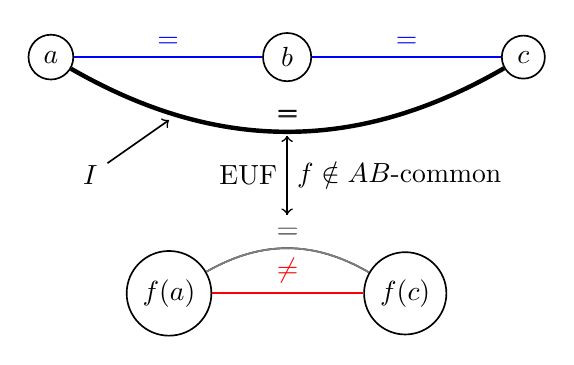
\begin{tikzpicture}[auto, node distance=3cm, semithick]
  \node [circle,draw] (a) at (0,3) {$a$};
  \node [circle,draw] (b) [right of=a] {$b$};
  \node [circle,draw] (c) [right of=b] {$c$};
  \node [circle,draw] (f_a) at (1.5,0) {$f(a)$};
  \node [circle,draw] (f_c) [right of=f_a] {$f(c)$};
  \path [draw=blue] (a) edge node {\textcolor{blue}{$=$}} (b);
  \path [draw=blue] (b) edge node {\textcolor{blue}{$=$}} (c);
  \path [draw=red] (f_a) edge node {\textcolor{red}{$\ne$}} (f_c);
  \visible<2-4>{\path (a) edge [bend right] node {$=$} (c);}
  \visible<3>{\path (f_a) edge [bend left] node {$=$} (f_c);}
  \visible<4->{\path [draw=gray] (f_a) edge [bend left] node {\textcolor{gray}{$=$}} (f_c);}
  \visible<3>{\draw [->] (3,2) to node[left] {EUF} (3,1);}
  \visible<4>{\draw [->] (3,1) to node[right] {$f \notin AB$-common} (3,2);}
  \visible<5->{
    \path [ultra thick] (a) edge [bend right] node {$=$} (c);
    \node [draw=none] (i) at (0.5,1.5) {$I$};
    \draw [->] (i) to (1.5,2.2);
  }

  \end{tikzpicture}
  \end{figure}
\end{frame}

\begin{frame}
  \frametitle{Interpolant for LA}
  \textcolor{blue}{$A \vec{x} \leq \vec{a}$} \hfill
  \textcolor{red}{$B \vec{x} \leq  \vec{b}$}
  \begin{figure}
  \centering
  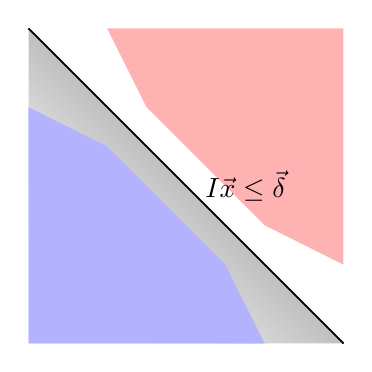
\begin{tikzpicture}[auto, node distance=3cm, semithick]
  \fill[blue!30!white] (0,0) -- (3,0) -- (2.5,1) -- (1,2.5) -- (0,3);
  \fill[red!30!white] (4,4) -- (1,4) -- (1.5,3) -- (3,1.5) -- (4,1);
  \visible<2>{\draw (0,4) to (4,0);}
  \visible<3->{
      \shadedraw[
        shading=axis,
        shading angle=-45,
        draw=none] (0,0) -- (4,0) -- (0,4) -- cycle;
      \fill[blue!30!white] (0,0) -- (3,0) -- (2.5,1) -- (1,2.5) -- (0,3);
      \draw (0,4) to node[right] {\mbox{}\ $I \vec{x} \leq \vec{\delta}$} (4,0);
  }
  \end{tikzpicture}
  \end{figure}
\end{frame}

%\begin{frame}
%  \frametitle{Applications}
%  \begin{itemize}
%  \item Predicate discovery for CEGAR-based model checkers\\
%        for refinement of abstract states.
%  \item Example: CSIsat is the new backend for \\
%        the software model checker \blast{}\footnote{[Henzinger 04] ~ \url{http://mtc.epfl.ch/software-tools/blast/}}:
%    \begin{itemize}
%    \item Improved dependencies and better compilation.
%    \item More comfortable for the user (no need to distinguish between
%      \foci{}\footnote{[McMillan 05] ~  \url{http://www.kenmcmil.com/foci.html}}
%      and \clpprover{}\footnote{[Rybalchenko 07] ~ \url{http://www.mpi-sws.mpg.de/~rybal/clp-prover/}} anymore).
%    \end{itemize}
%  \item Open-source software and freely extendable by others.
%  \end{itemize}
%\end{frame}

\begin{frame}
  \frametitle{Applications}
  \begin{itemize}
  \item Predicate discovery for CEGAR-based model checkers\\
        for refinement of abstract states.
  \item Example: %\csisat{} is the new backend for \\
        \blast{}\footnote{\url{http://mtc.epfl.ch/blast/}} 2.5 is based on \csisat{}:
    \begin{itemize}
      \item<2-> \foci{}\footnote{\url{http://www.kenmcmil.com/foci.html}} for DL + EUF.
      %\item<2-> \foci{}\footnote{[McMillan 05] ~  \url{http://www.kenmcmil.com/foci.html}} for DL + EUF.
      \item<3-> \clpprover{}\footnote{\url{http://www.mpi-sws.mpg.de/~rybal/clp-prover/}} for LA + EUF, but only conjunctions.
      %\item<3-> \clpprover{}\footnote{[Rybalchenko 07] ~ \url{http://www.mpi-sws.mpg.de/~rybal/clp-prover/}} for LA + EUF, but only conjunctions.
      \item<4-> \csisat{} is a new implementation for LA + EUF.
    \end{itemize}
  \item Open-source software and freely extendable by others.
    \begin{itemize}
    \item Total of 7500 lines of code written in Ocaml.
    \item Includes interpolation code and SMT solver.
    \end{itemize}
  \end{itemize}
\end{frame}

\section{How to use \csisat{} ?}
\begin{frame}
  \frametitle{What to give, what to expect}
  \begin{itemize}
  \item Input: $n$ formulae $X_1, \ldots, X_n$ such that
    \begin{equation*}
      \bigwedge_{i=1}^n X_i \models \bot
    \end{equation*}
  \item Output: $n-1$ interpolants such that
    \begin{eqnarray*}
      \bigwedge_{j=1}^i X_j & \models & I_i \\
      I_i \wedge \bigwedge_{j=i+1}^n X_j & \models & \bot
    \end{eqnarray*}
  \end{itemize}
\end{frame}

\begin{frame}[fragile]
  \frametitle{Syntax}
  \begin{itemize}
  \item Formula syntax is very simple and easy to integrate.
  \item \csisat{} supports also \foci{} syntax.
  \end{itemize}
  \vspace*{1cm}
  Example: \textcolor{blue}{$A$: ~ $a = b \wedge b = c$} ~~~~
  \textcolor{red}{$B$: ~ $f(a) \ne f(c)$}
  \begin{verbatim}
  a = b & b = c   ;    not  f(a) = f(c)
  \end{verbatim}
\end{frame}

\begin{frame}
  \frametitle{Example}
  \begin{figure}
  \centering
  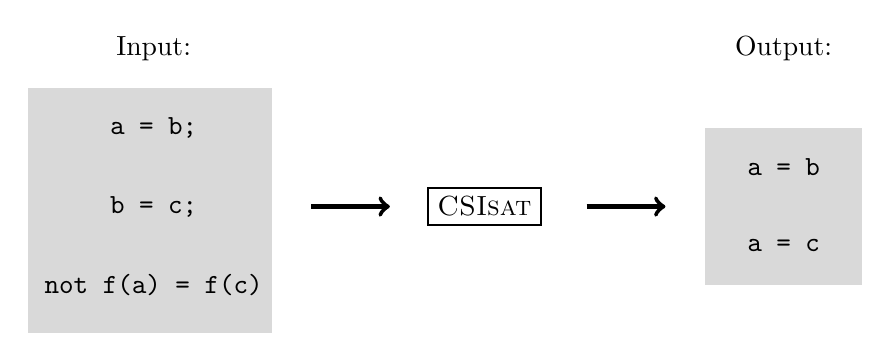
\begin{tikzpicture}[auto, node distance=3cm, semithick]
  \fill[black!15!white] (-1.6,-0.6) rectangle (1.5,2.5);
  \node [draw=none] (in) at (0,3) {Input:};
  \node [draw=none] (x1) at (0,2) {{\tt a = b;}};
  \node [draw=none] (x2) at (0,1) {{\tt b = c;}};
  \node [draw=none] (x3) at (0,0) {{\tt not f(a) = f(c)}};

  \visible<2->{
    \draw [->, ultra thick] (2,1) to (3,1);
    \node [thick,draw] (cs) at (4.2,1) {\csisat{}};
  }
  
  \visible<3->{
    \draw [->, ultra thick] (5.5,1) to (6.5,1);
    \fill[black!15!white] (7,0) rectangle (9,2);
    \node [draw=none] (out) at (8,3) {Output:};
    \node [draw=none] (i1) at (8,1.5) {{\tt a = b}};
    \node [draw=none] (i2) at (8,0.5) {{\tt a = c}};
  }

  \end{tikzpicture}
  \end{figure}
\end{frame}

\section{How \csisat{} works ?}
%\begin{frame}
%  \frametitle{General}
%  \csisat{} combines several known algorithms and provides them as open-source software.
%  \vspace{5pt}
%
%  \begin{tabular}{lcl}
%    Interpolation for EUF & $\rightarrow$ & McMillan 05\\
%    Interpolation for LA & $\rightarrow$ & Rybalchenko et al. 07\\
%    Interpolation using Nelson-Oppen & $\rightarrow$ &   Yorsh et al. 05\\
%     & + & Rybalchenko et al. 07\\
%    Interpolation with a resolution proof & $\rightarrow$  & Yorsh et al. 05
%  \end{tabular}
%
%\end{frame}

\begin{frame}
  \frametitle{Architecture}
  \begin{enumerate}
    \item Generating a resolution proof of unsatisfiability.
    \item<3-> Constructing the interpolant.
  \end{enumerate}

  \begin{figure}
  \centering
  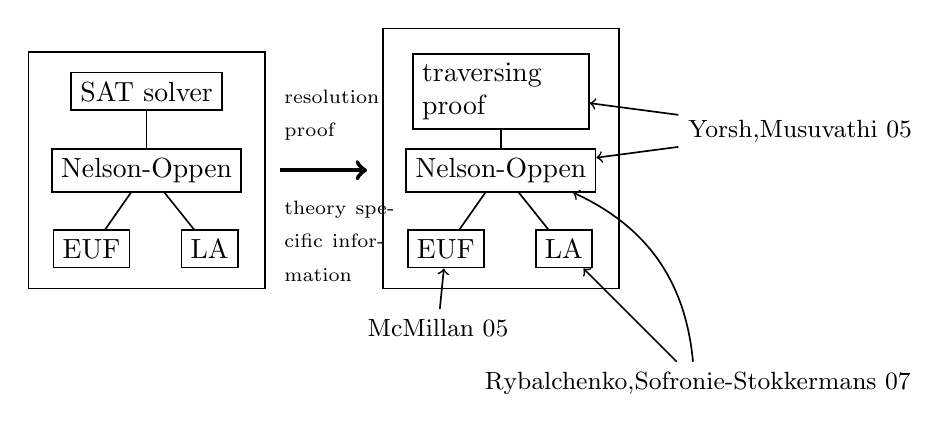
\begin{tikzpicture}[auto, node distance=3cm, semithick]

  \draw (-0.5,-0.5) rectangle (2.5,2.5);
  \node [draw] (sat) at (1,2) {SAT solver};
  \node [draw] (no) at (1,1) {Nelson-Oppen};
  \node [draw] (la) at (1.8,0) {LA};
  \node [draw] (euf) at (0.3,0) {EUF};
  \path (sat) edge (no);
  \path (no) edge (la);
  \path (no) edge (euf);

  \visible<2->{
    \draw [->, ultra thick] (2.7,1) to (3.8,1);
  }
  \visible<2>{
    \node [text width=15mm] (rp) at (3.5,1.7) {\scriptsize resolution proof};
    \node [text width=15mm] (uc) at (3.5,0.1) {\scriptsize theory specific information};
  }
  
  \visible<3->{
    \draw (4,-0.5) rectangle (7,2.8);
    \node [draw,text width=2cm] (trav) at (5.5,2) {traversing proof};
    \node [draw] (no2) at (5.5,1) {Nelson-Oppen};
    \node [draw] (la2) at (6.3,0) {LA};
    \node [draw] (euf2) at (4.8,0) {EUF};
    \path (trav) edge (no2);
    \path (no2) edge (la2);
    \path (no2) edge (euf2);
  }

  \visible<4->{
    \node (yorsh) at (9.3,1.5) {{\small Yorsh,Musuvathi 05}};
    \draw [->] (yorsh) edge  (trav);
  }

  \visible<5->{
    \node (rybal) at (8,-1.7) {{\small Rybalchenko,Sofronie-Stokkermans 07}};
    \draw [->] (yorsh) edge  (no2);
    \draw [->] (rybal) edge [bend right] (no2);
  }
  
  \visible<6->{
    \node (mcmill) at (4.7,-1) {{\small McMillan 05}};
    \draw [->] (mcmill) edge (euf2);
  }
  
  \visible<7->{
    \draw [->] (rybal) edge  (la2);
  }

  \end{tikzpicture}
  \end{figure}
\end{frame}

\section*{Conclusion}
\begin{frame}
  \frametitle{Performance}
  
\begin{figure}
{\footnotesize
\centering
\begin{tabular}{|l|rrrr|}
  \hline
  Program ~~~~~~~ &   \#queries  & ~ \foci{} & ~ \clpprover{}  & \textbf{~\csisat{}}     \\
  \hline
  \hline
  \blast{}\footnote{\url{http://mtc.epfl.ch/blast/}} & & & & \\
  floppy              &   235        & 1.17\,s    &  1.55\,s         & \textbf{0.55\,s}        \\
  cdaudio             &   130        & 0.60\,s    &  0.70\,s         & \textbf{0.26\,s}         \\
  ssh                 &  6881        & 29\,s      & ---              & \textbf{17\,s}         \\
  \hline
  \armc{}\footnote{\url{http://www.mpi-sws.mpg.de/~rybal/armc/}} & & & & \\
  magill      &  9860        & ---        & 30\,s            & \textbf{21\,s}         \\
  \hline
\end{tabular}
}
\end{figure}

\vspace{1cm}
{\footnotesize
Related work: the new version of \mathsat{} [CAV 08] can generate interpolants.
}

\end{frame}

\begin{frame}
  \frametitle{Try it out! }
  \csisat{} is freely available online:
  \begin{itemize}
    \item Project web page:\\ 
          \url{http://www.cs.sfu.ca/~dbeyer/CSIsat}
    \item Sources and bug reports:\\ 
          \url{http://csisat.googlecode.com}
    \item Feedback very welcome!
    \item[]
    \item Questions?
  \end{itemize}
\end{frame}
%-------------------------------------------------------------------------
%\bibliography{../../bib/sw,../../bib/tah}
%\documentclass{beamer}

% To have the citation lists ordered by number.
\usepackage[nocompress]{cite}
\usepackage[utf8]{inputenc}
\usepackage{graphicx}
\usepackage[tight,TABTOPCAP]{subfigure}
\usepackage{amsmath}
\usepackage{amssymb}
\usepackage{amsfonts}
\usepackage{url}

\usepackage{hyperref}

\usepackage{tikz}
\usepackage{color}

% Allow more than 70% (default) of a page to be filled by figures (100%).
\renewcommand\topfraction{1.0}

%%%%%%%%%% Tool Names %%%%%%%%%%%%
\newcommand{\csisat}{{\sc CSIsat}}
\newcommand{\blast}{{\sc Blast}}
\newcommand{\armc}{{\sc ARMC}}
\newcommand{\mathsat}{{\sc MathSAT}}
\newcommand{\picosat}{{\sc PicoSAT}}
\newcommand{\clpprover}{{\sc CLPprover}}
\newcommand{\foci}{{\sc Foci}}
\newcommand{\sicstus}{{\sc SICStus Prolog}}


%%%%%%%%%% NOTATIONS %%%%%%%%%%%%
\newcommand{\true}{{\it true}}
\newcommand{\false}{{\it false}}
\newcommand{\sat}{{\sc sat}}
\newcommand{\laeuf}{{\sc LA+EUF}}

\renewcommand{\implies}{\Rightarrow}


\hyphenation{CEGAR Blast sicstus prolog clpprover}

%TODO explain what is the CSIsat acronym ?
%DONE Craig citation
%DONE foci citation
%DONE clp citation
%DONE blast citation
%DONE slide number
%DONE name color (italic)
%DONE performance slide
%DONE related work MathSat
% inductive interpolant (Gregory), not needed (Tom)
%DONE syntax (infix)
%TODO application slide


\mode<presentation>
{
  \usetheme{Warsaw}
  %\usetheme{Frankfurt}
  % or ...

  %\setbeamercovered{transparent}
  % or whatever (possibly just delete it)
  %\setbeamertemplate{footline}[frame number]
  \useoutertheme{mysplit}
}
% Remove the navigation bar
\setbeamertemplate{navigation symbols}{}

\graphicspath{{./imgs/}}

\title[\csisat{}]{\csisat{}: Interpolation for \laeuf{}}

\AtBeginSection[]
{
  \begin{frame}<beamer>
    \frametitle{Outline}
    \tableofcontents[currentsection]
  \end{frame}
}

\author{Dirk Beyer\inst{1}     
\and 
        \textbf{Damien Zufferey}\inst{2}
%        \textcolor{blue}{Damien Zufferey}\inst{2}
\and 
        Rupak Majumdar\inst{3} 
}

\institute{
  ${}^1$ Simon Fraser University, BC, Canada \and
  ${}^2$ EPFL, Switzerland \and
  ${}^3$ UCLA, CA, USA   
}
\date{\vspace{5mm}\\ CAV'08, Princeton, ~~ July 11, 2008}

%-------------------------------------------------------------------------
\begin{document}

% Title
\frame[plain]{\titlepage}

\section*{Outline}
\begin{frame}
\tableofcontents
\end{frame}

\section{Interpolation}
\begin{frame}
  \frametitle{Definition [Craig 57]}
  Let $A$ and $B$ be two formulas such that
  $A \wedge B$ unsat.\\
  An interpolant $I$ has the following properties:
  \begin{itemize}
  \item $I$ contains only $AB$-common symbols.
  \item $A$ implies $I$
  \item $I \wedge B$ unsat.
  \end{itemize}
  Interpolation exists for $\text{\laeuf{}}$.
\end{frame}

\begin{frame}
%TODO b not in B
  \frametitle{Interpolant for EUF}
  \textcolor{blue}{$A$: ~~ $a = b \wedge b = c$} \hfill
  \textcolor{red}{$B$: ~~ $f(a) \ne f(c)$}
  \begin{figure}
  \centering
  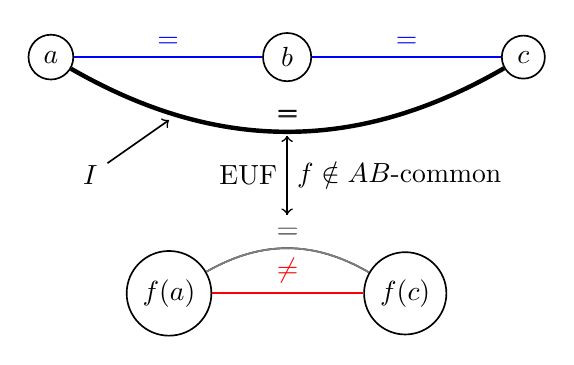
\begin{tikzpicture}[auto, node distance=3cm, semithick]
  \node [circle,draw] (a) at (0,3) {$a$};
  \node [circle,draw] (b) [right of=a] {$b$};
  \node [circle,draw] (c) [right of=b] {$c$};
  \node [circle,draw] (f_a) at (1.5,0) {$f(a)$};
  \node [circle,draw] (f_c) [right of=f_a] {$f(c)$};
  \path [draw=blue] (a) edge node {\textcolor{blue}{$=$}} (b);
  \path [draw=blue] (b) edge node {\textcolor{blue}{$=$}} (c);
  \path [draw=red] (f_a) edge node {\textcolor{red}{$\ne$}} (f_c);
  \visible<2-4>{\path (a) edge [bend right] node {$=$} (c);}
  \visible<3>{\path (f_a) edge [bend left] node {$=$} (f_c);}
  \visible<4->{\path [draw=gray] (f_a) edge [bend left] node {\textcolor{gray}{$=$}} (f_c);}
  \visible<3>{\draw [->] (3,2) to node[left] {EUF} (3,1);}
  \visible<4>{\draw [->] (3,1) to node[right] {$f \notin AB$-common} (3,2);}
  \visible<5->{
    \path [ultra thick] (a) edge [bend right] node {$=$} (c);
    \node [draw=none] (i) at (0.5,1.5) {$I$};
    \draw [->] (i) to (1.5,2.2);
  }

  \end{tikzpicture}
  \end{figure}
\end{frame}

\begin{frame}
  \frametitle{Interpolant for LA}
  \textcolor{blue}{$A \vec{x} \leq \vec{a}$} \hfill
  \textcolor{red}{$B \vec{x} \leq  \vec{b}$}
  \begin{figure}
  \centering
  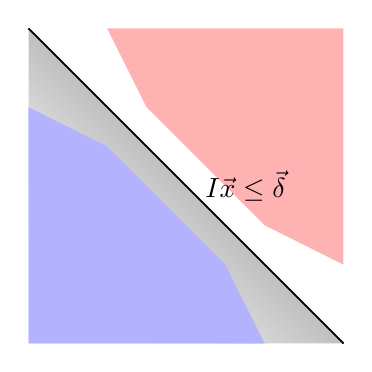
\begin{tikzpicture}[auto, node distance=3cm, semithick]
  \fill[blue!30!white] (0,0) -- (3,0) -- (2.5,1) -- (1,2.5) -- (0,3);
  \fill[red!30!white] (4,4) -- (1,4) -- (1.5,3) -- (3,1.5) -- (4,1);
  \visible<2>{\draw (0,4) to (4,0);}
  \visible<3->{
      \shadedraw[
        shading=axis,
        shading angle=-45,
        draw=none] (0,0) -- (4,0) -- (0,4) -- cycle;
      \fill[blue!30!white] (0,0) -- (3,0) -- (2.5,1) -- (1,2.5) -- (0,3);
      \draw (0,4) to node[right] {\mbox{}\ $I \vec{x} \leq \vec{\delta}$} (4,0);
  }
  \end{tikzpicture}
  \end{figure}
\end{frame}

%\begin{frame}
%  \frametitle{Applications}
%  \begin{itemize}
%  \item Predicate discovery for CEGAR-based model checkers\\
%        for refinement of abstract states.
%  \item Example: CSIsat is the new backend for \\
%        the software model checker \blast{}\footnote{[Henzinger 04] ~ \url{http://mtc.epfl.ch/software-tools/blast/}}:
%    \begin{itemize}
%    \item Improved dependencies and better compilation.
%    \item More comfortable for the user (no need to distinguish between
%      \foci{}\footnote{[McMillan 05] ~  \url{http://www.kenmcmil.com/foci.html}}
%      and \clpprover{}\footnote{[Rybalchenko 07] ~ \url{http://www.mpi-sws.mpg.de/~rybal/clp-prover/}} anymore).
%    \end{itemize}
%  \item Open-source software and freely extendable by others.
%  \end{itemize}
%\end{frame}

\begin{frame}
  \frametitle{Applications}
  \begin{itemize}
  \item Predicate discovery for CEGAR-based model checkers\\
        for refinement of abstract states.
  \item Example: %\csisat{} is the new backend for \\
        \blast{}\footnote{\url{http://mtc.epfl.ch/blast/}} 2.5 is based on \csisat{}:
    \begin{itemize}
      \item<2-> \foci{}\footnote{\url{http://www.kenmcmil.com/foci.html}} for DL + EUF.
      %\item<2-> \foci{}\footnote{[McMillan 05] ~  \url{http://www.kenmcmil.com/foci.html}} for DL + EUF.
      \item<3-> \clpprover{}\footnote{\url{http://www.mpi-sws.mpg.de/~rybal/clp-prover/}} for LA + EUF, but only conjunctions.
      %\item<3-> \clpprover{}\footnote{[Rybalchenko 07] ~ \url{http://www.mpi-sws.mpg.de/~rybal/clp-prover/}} for LA + EUF, but only conjunctions.
      \item<4-> \csisat{} is a new implementation for LA + EUF.
    \end{itemize}
  \item Open-source software and freely extendable by others.
    \begin{itemize}
    \item Total of 7500 lines of code written in Ocaml.
    \item Includes interpolation code and SMT solver.
    \end{itemize}
  \end{itemize}
\end{frame}

\section{How to use \csisat{} ?}
\begin{frame}
  \frametitle{What to give, what to expect}
  \begin{itemize}
  \item Input: $n$ formulae $X_1, \ldots, X_n$ such that
    \begin{equation*}
      \bigwedge_{i=1}^n X_i \models \bot
    \end{equation*}
  \item Output: $n-1$ interpolants such that
    \begin{eqnarray*}
      \bigwedge_{j=1}^i X_j & \models & I_i \\
      I_i \wedge \bigwedge_{j=i+1}^n X_j & \models & \bot
    \end{eqnarray*}
  \end{itemize}
\end{frame}

\begin{frame}[fragile]
  \frametitle{Syntax}
  \begin{itemize}
  \item Formula syntax is very simple and easy to integrate.
  \item \csisat{} supports also \foci{} syntax.
  \end{itemize}
  \vspace*{1cm}
  Example: \textcolor{blue}{$A$: ~ $a = b \wedge b = c$} ~~~~
  \textcolor{red}{$B$: ~ $f(a) \ne f(c)$}
  \begin{verbatim}
  a = b & b = c   ;    not  f(a) = f(c)
  \end{verbatim}
\end{frame}

\begin{frame}
  \frametitle{Example}
  \begin{figure}
  \centering
  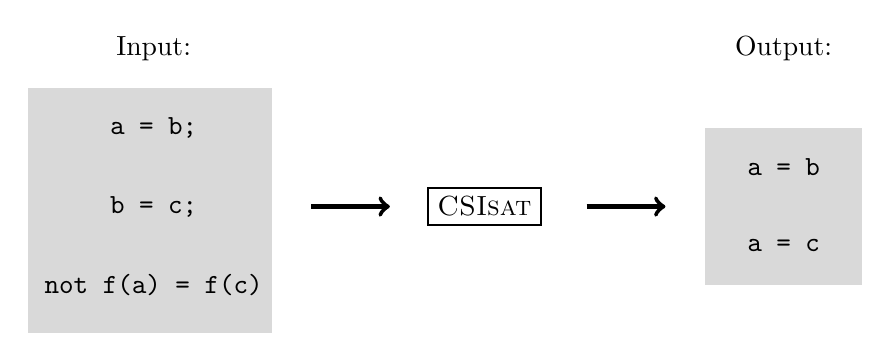
\begin{tikzpicture}[auto, node distance=3cm, semithick]
  \fill[black!15!white] (-1.6,-0.6) rectangle (1.5,2.5);
  \node [draw=none] (in) at (0,3) {Input:};
  \node [draw=none] (x1) at (0,2) {{\tt a = b;}};
  \node [draw=none] (x2) at (0,1) {{\tt b = c;}};
  \node [draw=none] (x3) at (0,0) {{\tt not f(a) = f(c)}};

  \visible<2->{
    \draw [->, ultra thick] (2,1) to (3,1);
    \node [thick,draw] (cs) at (4.2,1) {\csisat{}};
  }
  
  \visible<3->{
    \draw [->, ultra thick] (5.5,1) to (6.5,1);
    \fill[black!15!white] (7,0) rectangle (9,2);
    \node [draw=none] (out) at (8,3) {Output:};
    \node [draw=none] (i1) at (8,1.5) {{\tt a = b}};
    \node [draw=none] (i2) at (8,0.5) {{\tt a = c}};
  }

  \end{tikzpicture}
  \end{figure}
\end{frame}

\section{How \csisat{} works ?}
%\begin{frame}
%  \frametitle{General}
%  \csisat{} combines several known algorithms and provides them as open-source software.
%  \vspace{5pt}
%
%  \begin{tabular}{lcl}
%    Interpolation for EUF & $\rightarrow$ & McMillan 05\\
%    Interpolation for LA & $\rightarrow$ & Rybalchenko et al. 07\\
%    Interpolation using Nelson-Oppen & $\rightarrow$ &   Yorsh et al. 05\\
%     & + & Rybalchenko et al. 07\\
%    Interpolation with a resolution proof & $\rightarrow$  & Yorsh et al. 05
%  \end{tabular}
%
%\end{frame}

\begin{frame}
  \frametitle{Architecture}
  \begin{enumerate}
    \item Generating a resolution proof of unsatisfiability.
    \item<3-> Constructing the interpolant.
  \end{enumerate}

  \begin{figure}
  \centering
  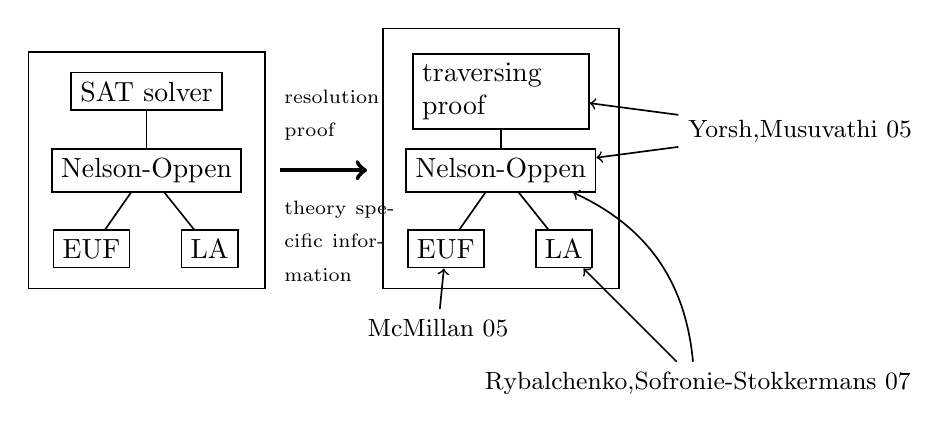
\begin{tikzpicture}[auto, node distance=3cm, semithick]

  \draw (-0.5,-0.5) rectangle (2.5,2.5);
  \node [draw] (sat) at (1,2) {SAT solver};
  \node [draw] (no) at (1,1) {Nelson-Oppen};
  \node [draw] (la) at (1.8,0) {LA};
  \node [draw] (euf) at (0.3,0) {EUF};
  \path (sat) edge (no);
  \path (no) edge (la);
  \path (no) edge (euf);

  \visible<2->{
    \draw [->, ultra thick] (2.7,1) to (3.8,1);
  }
  \visible<2>{
    \node [text width=15mm] (rp) at (3.5,1.7) {\scriptsize resolution proof};
    \node [text width=15mm] (uc) at (3.5,0.1) {\scriptsize theory specific information};
  }
  
  \visible<3->{
    \draw (4,-0.5) rectangle (7,2.8);
    \node [draw,text width=2cm] (trav) at (5.5,2) {traversing proof};
    \node [draw] (no2) at (5.5,1) {Nelson-Oppen};
    \node [draw] (la2) at (6.3,0) {LA};
    \node [draw] (euf2) at (4.8,0) {EUF};
    \path (trav) edge (no2);
    \path (no2) edge (la2);
    \path (no2) edge (euf2);
  }

  \visible<4->{
    \node (yorsh) at (9.3,1.5) {{\small Yorsh,Musuvathi 05}};
    \draw [->] (yorsh) edge  (trav);
  }

  \visible<5->{
    \node (rybal) at (8,-1.7) {{\small Rybalchenko,Sofronie-Stokkermans 07}};
    \draw [->] (yorsh) edge  (no2);
    \draw [->] (rybal) edge [bend right] (no2);
  }
  
  \visible<6->{
    \node (mcmill) at (4.7,-1) {{\small McMillan 05}};
    \draw [->] (mcmill) edge (euf2);
  }
  
  \visible<7->{
    \draw [->] (rybal) edge  (la2);
  }

  \end{tikzpicture}
  \end{figure}
\end{frame}

\section*{Conclusion}
\begin{frame}
  \frametitle{Performance}
  
\begin{figure}
{\footnotesize
\centering
\begin{tabular}{|l|rrrr|}
  \hline
  Program ~~~~~~~ &   \#queries  & ~ \foci{} & ~ \clpprover{}  & \textbf{~\csisat{}}     \\
  \hline
  \hline
  \blast{}\footnote{\url{http://mtc.epfl.ch/blast/}} & & & & \\
  floppy              &   235        & 1.17\,s    &  1.55\,s         & \textbf{0.55\,s}        \\
  cdaudio             &   130        & 0.60\,s    &  0.70\,s         & \textbf{0.26\,s}         \\
  ssh                 &  6881        & 29\,s      & ---              & \textbf{17\,s}         \\
  \hline
  \armc{}\footnote{\url{http://www.mpi-sws.mpg.de/~rybal/armc/}} & & & & \\
  magill      &  9860        & ---        & 30\,s            & \textbf{21\,s}         \\
  \hline
\end{tabular}
}
\end{figure}

\vspace{1cm}
{\footnotesize
Related work: the new version of \mathsat{} [CAV 08] can generate interpolants.
}

\end{frame}

\begin{frame}
  \frametitle{Try it out! }
  \csisat{} is freely available online:
  \begin{itemize}
    \item Project web page:\\ 
          \url{http://www.cs.sfu.ca/~dbeyer/CSIsat}
    \item Sources and bug reports:\\ 
          \url{http://csisat.googlecode.com}
    \item Feedback very welcome!
    \item[]
    \item Questions?
  \end{itemize}
\end{frame}
%-------------------------------------------------------------------------
%\bibliography{../../bib/sw,../../bib/tah}
%\documentclass{beamer}

% To have the citation lists ordered by number.
\usepackage[nocompress]{cite}
\usepackage[utf8]{inputenc}
\usepackage{graphicx}
\usepackage[tight,TABTOPCAP]{subfigure}
\usepackage{amsmath}
\usepackage{amssymb}
\usepackage{amsfonts}
\usepackage{url}

\usepackage{hyperref}

\usepackage{tikz}
\usepackage{color}

% Allow more than 70% (default) of a page to be filled by figures (100%).
\renewcommand\topfraction{1.0}

%%%%%%%%%% Tool Names %%%%%%%%%%%%
\newcommand{\csisat}{{\sc CSIsat}}
\newcommand{\blast}{{\sc Blast}}
\newcommand{\armc}{{\sc ARMC}}
\newcommand{\mathsat}{{\sc MathSAT}}
\newcommand{\picosat}{{\sc PicoSAT}}
\newcommand{\clpprover}{{\sc CLPprover}}
\newcommand{\foci}{{\sc Foci}}
\newcommand{\sicstus}{{\sc SICStus Prolog}}


%%%%%%%%%% NOTATIONS %%%%%%%%%%%%
\newcommand{\true}{{\it true}}
\newcommand{\false}{{\it false}}
\newcommand{\sat}{{\sc sat}}
\newcommand{\laeuf}{{\sc LA+EUF}}

\renewcommand{\implies}{\Rightarrow}


\hyphenation{CEGAR Blast sicstus prolog clpprover}

%TODO explain what is the CSIsat acronym ?
%DONE Craig citation
%DONE foci citation
%DONE clp citation
%DONE blast citation
%DONE slide number
%DONE name color (italic)
%DONE performance slide
%DONE related work MathSat
% inductive interpolant (Gregory), not needed (Tom)
%DONE syntax (infix)
%TODO application slide


\mode<presentation>
{
  \usetheme{Warsaw}
  %\usetheme{Frankfurt}
  % or ...

  %\setbeamercovered{transparent}
  % or whatever (possibly just delete it)
  %\setbeamertemplate{footline}[frame number]
  \useoutertheme{mysplit}
}
% Remove the navigation bar
\setbeamertemplate{navigation symbols}{}

\graphicspath{{./imgs/}}

\title[\csisat{}]{\csisat{}: Interpolation for \laeuf{}}

\AtBeginSection[]
{
  \begin{frame}<beamer>
    \frametitle{Outline}
    \tableofcontents[currentsection]
  \end{frame}
}

\author{Dirk Beyer\inst{1}     
\and 
        \textbf{Damien Zufferey}\inst{2}
%        \textcolor{blue}{Damien Zufferey}\inst{2}
\and 
        Rupak Majumdar\inst{3} 
}

\institute{
  ${}^1$ Simon Fraser University, BC, Canada \and
  ${}^2$ EPFL, Switzerland \and
  ${}^3$ UCLA, CA, USA   
}
\date{\vspace{5mm}\\ CAV'08, Princeton, ~~ July 11, 2008}

%-------------------------------------------------------------------------
\begin{document}

% Title
\frame[plain]{\titlepage}

\section*{Outline}
\begin{frame}
\tableofcontents
\end{frame}

\section{Interpolation}
\begin{frame}
  \frametitle{Definition [Craig 57]}
  Let $A$ and $B$ be two formulas such that
  $A \wedge B$ unsat.\\
  An interpolant $I$ has the following properties:
  \begin{itemize}
  \item $I$ contains only $AB$-common symbols.
  \item $A$ implies $I$
  \item $I \wedge B$ unsat.
  \end{itemize}
  Interpolation exists for $\text{\laeuf{}}$.
\end{frame}

\begin{frame}
%TODO b not in B
  \frametitle{Interpolant for EUF}
  \textcolor{blue}{$A$: ~~ $a = b \wedge b = c$} \hfill
  \textcolor{red}{$B$: ~~ $f(a) \ne f(c)$}
  \begin{figure}
  \centering
  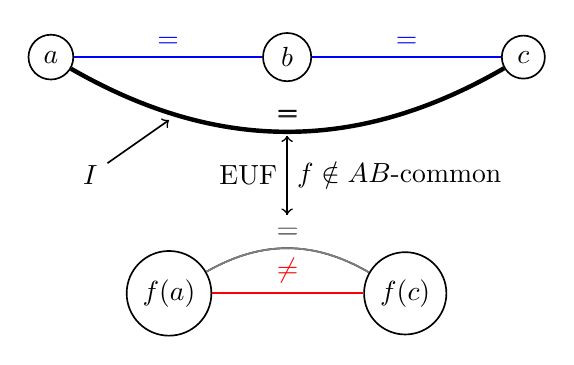
\begin{tikzpicture}[auto, node distance=3cm, semithick]
  \node [circle,draw] (a) at (0,3) {$a$};
  \node [circle,draw] (b) [right of=a] {$b$};
  \node [circle,draw] (c) [right of=b] {$c$};
  \node [circle,draw] (f_a) at (1.5,0) {$f(a)$};
  \node [circle,draw] (f_c) [right of=f_a] {$f(c)$};
  \path [draw=blue] (a) edge node {\textcolor{blue}{$=$}} (b);
  \path [draw=blue] (b) edge node {\textcolor{blue}{$=$}} (c);
  \path [draw=red] (f_a) edge node {\textcolor{red}{$\ne$}} (f_c);
  \visible<2-4>{\path (a) edge [bend right] node {$=$} (c);}
  \visible<3>{\path (f_a) edge [bend left] node {$=$} (f_c);}
  \visible<4->{\path [draw=gray] (f_a) edge [bend left] node {\textcolor{gray}{$=$}} (f_c);}
  \visible<3>{\draw [->] (3,2) to node[left] {EUF} (3,1);}
  \visible<4>{\draw [->] (3,1) to node[right] {$f \notin AB$-common} (3,2);}
  \visible<5->{
    \path [ultra thick] (a) edge [bend right] node {$=$} (c);
    \node [draw=none] (i) at (0.5,1.5) {$I$};
    \draw [->] (i) to (1.5,2.2);
  }

  \end{tikzpicture}
  \end{figure}
\end{frame}

\begin{frame}
  \frametitle{Interpolant for LA}
  \textcolor{blue}{$A \vec{x} \leq \vec{a}$} \hfill
  \textcolor{red}{$B \vec{x} \leq  \vec{b}$}
  \begin{figure}
  \centering
  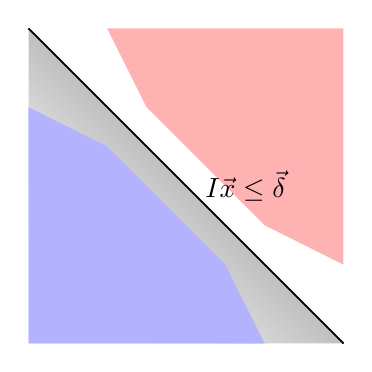
\begin{tikzpicture}[auto, node distance=3cm, semithick]
  \fill[blue!30!white] (0,0) -- (3,0) -- (2.5,1) -- (1,2.5) -- (0,3);
  \fill[red!30!white] (4,4) -- (1,4) -- (1.5,3) -- (3,1.5) -- (4,1);
  \visible<2>{\draw (0,4) to (4,0);}
  \visible<3->{
      \shadedraw[
        shading=axis,
        shading angle=-45,
        draw=none] (0,0) -- (4,0) -- (0,4) -- cycle;
      \fill[blue!30!white] (0,0) -- (3,0) -- (2.5,1) -- (1,2.5) -- (0,3);
      \draw (0,4) to node[right] {\mbox{}\ $I \vec{x} \leq \vec{\delta}$} (4,0);
  }
  \end{tikzpicture}
  \end{figure}
\end{frame}

%\begin{frame}
%  \frametitle{Applications}
%  \begin{itemize}
%  \item Predicate discovery for CEGAR-based model checkers\\
%        for refinement of abstract states.
%  \item Example: CSIsat is the new backend for \\
%        the software model checker \blast{}\footnote{[Henzinger 04] ~ \url{http://mtc.epfl.ch/software-tools/blast/}}:
%    \begin{itemize}
%    \item Improved dependencies and better compilation.
%    \item More comfortable for the user (no need to distinguish between
%      \foci{}\footnote{[McMillan 05] ~  \url{http://www.kenmcmil.com/foci.html}}
%      and \clpprover{}\footnote{[Rybalchenko 07] ~ \url{http://www.mpi-sws.mpg.de/~rybal/clp-prover/}} anymore).
%    \end{itemize}
%  \item Open-source software and freely extendable by others.
%  \end{itemize}
%\end{frame}

\begin{frame}
  \frametitle{Applications}
  \begin{itemize}
  \item Predicate discovery for CEGAR-based model checkers\\
        for refinement of abstract states.
  \item Example: %\csisat{} is the new backend for \\
        \blast{}\footnote{\url{http://mtc.epfl.ch/blast/}} 2.5 is based on \csisat{}:
    \begin{itemize}
      \item<2-> \foci{}\footnote{\url{http://www.kenmcmil.com/foci.html}} for DL + EUF.
      %\item<2-> \foci{}\footnote{[McMillan 05] ~  \url{http://www.kenmcmil.com/foci.html}} for DL + EUF.
      \item<3-> \clpprover{}\footnote{\url{http://www.mpi-sws.mpg.de/~rybal/clp-prover/}} for LA + EUF, but only conjunctions.
      %\item<3-> \clpprover{}\footnote{[Rybalchenko 07] ~ \url{http://www.mpi-sws.mpg.de/~rybal/clp-prover/}} for LA + EUF, but only conjunctions.
      \item<4-> \csisat{} is a new implementation for LA + EUF.
    \end{itemize}
  \item Open-source software and freely extendable by others.
    \begin{itemize}
    \item Total of 7500 lines of code written in Ocaml.
    \item Includes interpolation code and SMT solver.
    \end{itemize}
  \end{itemize}
\end{frame}

\section{How to use \csisat{} ?}
\begin{frame}
  \frametitle{What to give, what to expect}
  \begin{itemize}
  \item Input: $n$ formulae $X_1, \ldots, X_n$ such that
    \begin{equation*}
      \bigwedge_{i=1}^n X_i \models \bot
    \end{equation*}
  \item Output: $n-1$ interpolants such that
    \begin{eqnarray*}
      \bigwedge_{j=1}^i X_j & \models & I_i \\
      I_i \wedge \bigwedge_{j=i+1}^n X_j & \models & \bot
    \end{eqnarray*}
  \end{itemize}
\end{frame}

\begin{frame}[fragile]
  \frametitle{Syntax}
  \begin{itemize}
  \item Formula syntax is very simple and easy to integrate.
  \item \csisat{} supports also \foci{} syntax.
  \end{itemize}
  \vspace*{1cm}
  Example: \textcolor{blue}{$A$: ~ $a = b \wedge b = c$} ~~~~
  \textcolor{red}{$B$: ~ $f(a) \ne f(c)$}
  \begin{verbatim}
  a = b & b = c   ;    not  f(a) = f(c)
  \end{verbatim}
\end{frame}

\begin{frame}
  \frametitle{Example}
  \begin{figure}
  \centering
  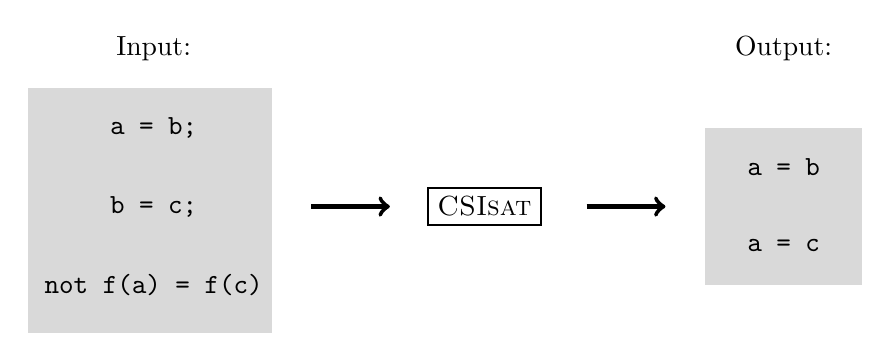
\begin{tikzpicture}[auto, node distance=3cm, semithick]
  \fill[black!15!white] (-1.6,-0.6) rectangle (1.5,2.5);
  \node [draw=none] (in) at (0,3) {Input:};
  \node [draw=none] (x1) at (0,2) {{\tt a = b;}};
  \node [draw=none] (x2) at (0,1) {{\tt b = c;}};
  \node [draw=none] (x3) at (0,0) {{\tt not f(a) = f(c)}};

  \visible<2->{
    \draw [->, ultra thick] (2,1) to (3,1);
    \node [thick,draw] (cs) at (4.2,1) {\csisat{}};
  }
  
  \visible<3->{
    \draw [->, ultra thick] (5.5,1) to (6.5,1);
    \fill[black!15!white] (7,0) rectangle (9,2);
    \node [draw=none] (out) at (8,3) {Output:};
    \node [draw=none] (i1) at (8,1.5) {{\tt a = b}};
    \node [draw=none] (i2) at (8,0.5) {{\tt a = c}};
  }

  \end{tikzpicture}
  \end{figure}
\end{frame}

\section{How \csisat{} works ?}
%\begin{frame}
%  \frametitle{General}
%  \csisat{} combines several known algorithms and provides them as open-source software.
%  \vspace{5pt}
%
%  \begin{tabular}{lcl}
%    Interpolation for EUF & $\rightarrow$ & McMillan 05\\
%    Interpolation for LA & $\rightarrow$ & Rybalchenko et al. 07\\
%    Interpolation using Nelson-Oppen & $\rightarrow$ &   Yorsh et al. 05\\
%     & + & Rybalchenko et al. 07\\
%    Interpolation with a resolution proof & $\rightarrow$  & Yorsh et al. 05
%  \end{tabular}
%
%\end{frame}

\begin{frame}
  \frametitle{Architecture}
  \begin{enumerate}
    \item Generating a resolution proof of unsatisfiability.
    \item<3-> Constructing the interpolant.
  \end{enumerate}

  \begin{figure}
  \centering
  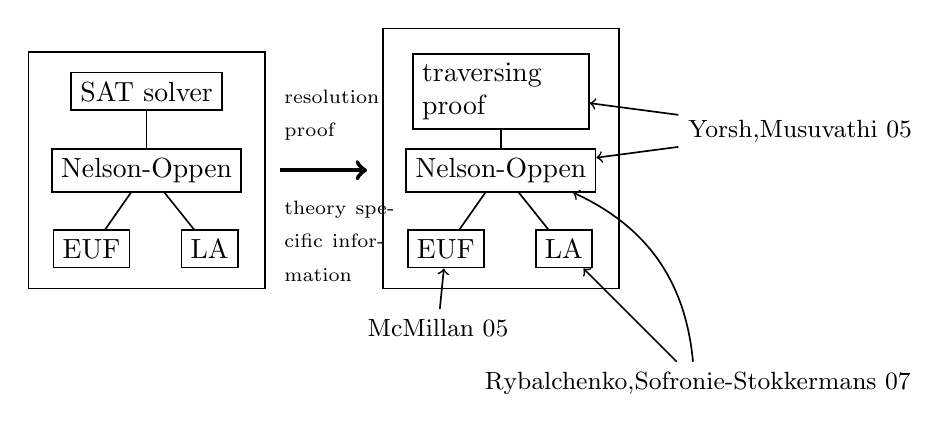
\begin{tikzpicture}[auto, node distance=3cm, semithick]

  \draw (-0.5,-0.5) rectangle (2.5,2.5);
  \node [draw] (sat) at (1,2) {SAT solver};
  \node [draw] (no) at (1,1) {Nelson-Oppen};
  \node [draw] (la) at (1.8,0) {LA};
  \node [draw] (euf) at (0.3,0) {EUF};
  \path (sat) edge (no);
  \path (no) edge (la);
  \path (no) edge (euf);

  \visible<2->{
    \draw [->, ultra thick] (2.7,1) to (3.8,1);
  }
  \visible<2>{
    \node [text width=15mm] (rp) at (3.5,1.7) {\scriptsize resolution proof};
    \node [text width=15mm] (uc) at (3.5,0.1) {\scriptsize theory specific information};
  }
  
  \visible<3->{
    \draw (4,-0.5) rectangle (7,2.8);
    \node [draw,text width=2cm] (trav) at (5.5,2) {traversing proof};
    \node [draw] (no2) at (5.5,1) {Nelson-Oppen};
    \node [draw] (la2) at (6.3,0) {LA};
    \node [draw] (euf2) at (4.8,0) {EUF};
    \path (trav) edge (no2);
    \path (no2) edge (la2);
    \path (no2) edge (euf2);
  }

  \visible<4->{
    \node (yorsh) at (9.3,1.5) {{\small Yorsh,Musuvathi 05}};
    \draw [->] (yorsh) edge  (trav);
  }

  \visible<5->{
    \node (rybal) at (8,-1.7) {{\small Rybalchenko,Sofronie-Stokkermans 07}};
    \draw [->] (yorsh) edge  (no2);
    \draw [->] (rybal) edge [bend right] (no2);
  }
  
  \visible<6->{
    \node (mcmill) at (4.7,-1) {{\small McMillan 05}};
    \draw [->] (mcmill) edge (euf2);
  }
  
  \visible<7->{
    \draw [->] (rybal) edge  (la2);
  }

  \end{tikzpicture}
  \end{figure}
\end{frame}

\section*{Conclusion}
\begin{frame}
  \frametitle{Performance}
  
\begin{figure}
{\footnotesize
\centering
\begin{tabular}{|l|rrrr|}
  \hline
  Program ~~~~~~~ &   \#queries  & ~ \foci{} & ~ \clpprover{}  & \textbf{~\csisat{}}     \\
  \hline
  \hline
  \blast{}\footnote{\url{http://mtc.epfl.ch/blast/}} & & & & \\
  floppy              &   235        & 1.17\,s    &  1.55\,s         & \textbf{0.55\,s}        \\
  cdaudio             &   130        & 0.60\,s    &  0.70\,s         & \textbf{0.26\,s}         \\
  ssh                 &  6881        & 29\,s      & ---              & \textbf{17\,s}         \\
  \hline
  \armc{}\footnote{\url{http://www.mpi-sws.mpg.de/~rybal/armc/}} & & & & \\
  magill      &  9860        & ---        & 30\,s            & \textbf{21\,s}         \\
  \hline
\end{tabular}
}
\end{figure}

\vspace{1cm}
{\footnotesize
Related work: the new version of \mathsat{} [CAV 08] can generate interpolants.
}

\end{frame}

\begin{frame}
  \frametitle{Try it out! }
  \csisat{} is freely available online:
  \begin{itemize}
    \item Project web page:\\ 
          \url{http://www.cs.sfu.ca/~dbeyer/CSIsat}
    \item Sources and bug reports:\\ 
          \url{http://csisat.googlecode.com}
    \item Feedback very welcome!
    \item[]
    \item Questions?
  \end{itemize}
\end{frame}
%-------------------------------------------------------------------------
%\bibliography{../../bib/sw,../../bib/tah}
%\documentclass{beamer}

% To have the citation lists ordered by number.
\usepackage[nocompress]{cite}
\usepackage[utf8]{inputenc}
\usepackage{graphicx}
\usepackage[tight,TABTOPCAP]{subfigure}
\usepackage{amsmath}
\usepackage{amssymb}
\usepackage{amsfonts}
\usepackage{url}

\usepackage{hyperref}

\usepackage{tikz}
\usepackage{color}

% Allow more than 70% (default) of a page to be filled by figures (100%).
\renewcommand\topfraction{1.0}

%%%%%%%%%% Tool Names %%%%%%%%%%%%
\newcommand{\csisat}{{\sc CSIsat}}
\newcommand{\blast}{{\sc Blast}}
\newcommand{\armc}{{\sc ARMC}}
\newcommand{\mathsat}{{\sc MathSAT}}
\newcommand{\picosat}{{\sc PicoSAT}}
\newcommand{\clpprover}{{\sc CLPprover}}
\newcommand{\foci}{{\sc Foci}}
\newcommand{\sicstus}{{\sc SICStus Prolog}}


%%%%%%%%%% NOTATIONS %%%%%%%%%%%%
\newcommand{\true}{{\it true}}
\newcommand{\false}{{\it false}}
\newcommand{\sat}{{\sc sat}}
\newcommand{\laeuf}{{\sc LA+EUF}}

\renewcommand{\implies}{\Rightarrow}


\hyphenation{CEGAR Blast sicstus prolog clpprover}

%TODO explain what is the CSIsat acronym ?
%DONE Craig citation
%DONE foci citation
%DONE clp citation
%DONE blast citation
%DONE slide number
%DONE name color (italic)
%DONE performance slide
%DONE related work MathSat
% inductive interpolant (Gregory), not needed (Tom)
%DONE syntax (infix)
%TODO application slide


\mode<presentation>
{
  \usetheme{Warsaw}
  %\usetheme{Frankfurt}
  % or ...

  %\setbeamercovered{transparent}
  % or whatever (possibly just delete it)
  %\setbeamertemplate{footline}[frame number]
  \useoutertheme{mysplit}
}
% Remove the navigation bar
\setbeamertemplate{navigation symbols}{}

\graphicspath{{./imgs/}}

\title[\csisat{}]{\csisat{}: Interpolation for \laeuf{}}

\AtBeginSection[]
{
  \begin{frame}<beamer>
    \frametitle{Outline}
    \tableofcontents[currentsection]
  \end{frame}
}

\author{Dirk Beyer\inst{1}     
\and 
        \textbf{Damien Zufferey}\inst{2}
%        \textcolor{blue}{Damien Zufferey}\inst{2}
\and 
        Rupak Majumdar\inst{3} 
}

\institute{
  ${}^1$ Simon Fraser University, BC, Canada \and
  ${}^2$ EPFL, Switzerland \and
  ${}^3$ UCLA, CA, USA   
}
\date{\vspace{5mm}\\ CAV'08, Princeton, ~~ July 11, 2008}

%-------------------------------------------------------------------------
\begin{document}

% Title
\frame[plain]{\titlepage}

\section*{Outline}
\begin{frame}
\tableofcontents
\end{frame}

\section{Interpolation}
\begin{frame}
  \frametitle{Definition [Craig 57]}
  Let $A$ and $B$ be two formulas such that
  $A \wedge B$ unsat.\\
  An interpolant $I$ has the following properties:
  \begin{itemize}
  \item $I$ contains only $AB$-common symbols.
  \item $A$ implies $I$
  \item $I \wedge B$ unsat.
  \end{itemize}
  Interpolation exists for $\text{\laeuf{}}$.
\end{frame}

\begin{frame}
%TODO b not in B
  \frametitle{Interpolant for EUF}
  \textcolor{blue}{$A$: ~~ $a = b \wedge b = c$} \hfill
  \textcolor{red}{$B$: ~~ $f(a) \ne f(c)$}
  \begin{figure}
  \centering
  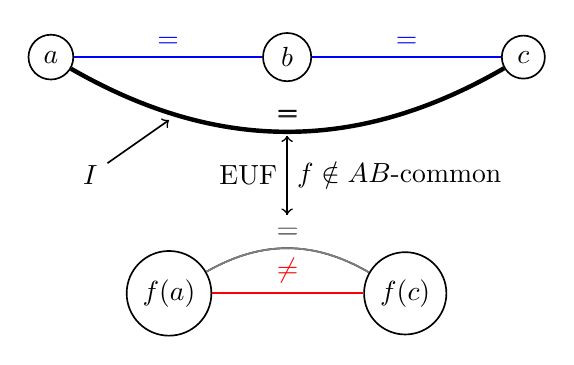
\begin{tikzpicture}[auto, node distance=3cm, semithick]
  \node [circle,draw] (a) at (0,3) {$a$};
  \node [circle,draw] (b) [right of=a] {$b$};
  \node [circle,draw] (c) [right of=b] {$c$};
  \node [circle,draw] (f_a) at (1.5,0) {$f(a)$};
  \node [circle,draw] (f_c) [right of=f_a] {$f(c)$};
  \path [draw=blue] (a) edge node {\textcolor{blue}{$=$}} (b);
  \path [draw=blue] (b) edge node {\textcolor{blue}{$=$}} (c);
  \path [draw=red] (f_a) edge node {\textcolor{red}{$\ne$}} (f_c);
  \visible<2-4>{\path (a) edge [bend right] node {$=$} (c);}
  \visible<3>{\path (f_a) edge [bend left] node {$=$} (f_c);}
  \visible<4->{\path [draw=gray] (f_a) edge [bend left] node {\textcolor{gray}{$=$}} (f_c);}
  \visible<3>{\draw [->] (3,2) to node[left] {EUF} (3,1);}
  \visible<4>{\draw [->] (3,1) to node[right] {$f \notin AB$-common} (3,2);}
  \visible<5->{
    \path [ultra thick] (a) edge [bend right] node {$=$} (c);
    \node [draw=none] (i) at (0.5,1.5) {$I$};
    \draw [->] (i) to (1.5,2.2);
  }

  \end{tikzpicture}
  \end{figure}
\end{frame}

\begin{frame}
  \frametitle{Interpolant for LA}
  \textcolor{blue}{$A \vec{x} \leq \vec{a}$} \hfill
  \textcolor{red}{$B \vec{x} \leq  \vec{b}$}
  \begin{figure}
  \centering
  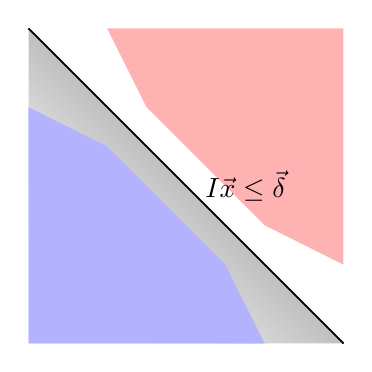
\begin{tikzpicture}[auto, node distance=3cm, semithick]
  \fill[blue!30!white] (0,0) -- (3,0) -- (2.5,1) -- (1,2.5) -- (0,3);
  \fill[red!30!white] (4,4) -- (1,4) -- (1.5,3) -- (3,1.5) -- (4,1);
  \visible<2>{\draw (0,4) to (4,0);}
  \visible<3->{
      \shadedraw[
        shading=axis,
        shading angle=-45,
        draw=none] (0,0) -- (4,0) -- (0,4) -- cycle;
      \fill[blue!30!white] (0,0) -- (3,0) -- (2.5,1) -- (1,2.5) -- (0,3);
      \draw (0,4) to node[right] {\mbox{}\ $I \vec{x} \leq \vec{\delta}$} (4,0);
  }
  \end{tikzpicture}
  \end{figure}
\end{frame}

%\begin{frame}
%  \frametitle{Applications}
%  \begin{itemize}
%  \item Predicate discovery for CEGAR-based model checkers\\
%        for refinement of abstract states.
%  \item Example: CSIsat is the new backend for \\
%        the software model checker \blast{}\footnote{[Henzinger 04] ~ \url{http://mtc.epfl.ch/software-tools/blast/}}:
%    \begin{itemize}
%    \item Improved dependencies and better compilation.
%    \item More comfortable for the user (no need to distinguish between
%      \foci{}\footnote{[McMillan 05] ~  \url{http://www.kenmcmil.com/foci.html}}
%      and \clpprover{}\footnote{[Rybalchenko 07] ~ \url{http://www.mpi-sws.mpg.de/~rybal/clp-prover/}} anymore).
%    \end{itemize}
%  \item Open-source software and freely extendable by others.
%  \end{itemize}
%\end{frame}

\begin{frame}
  \frametitle{Applications}
  \begin{itemize}
  \item Predicate discovery for CEGAR-based model checkers\\
        for refinement of abstract states.
  \item Example: %\csisat{} is the new backend for \\
        \blast{}\footnote{\url{http://mtc.epfl.ch/blast/}} 2.5 is based on \csisat{}:
    \begin{itemize}
      \item<2-> \foci{}\footnote{\url{http://www.kenmcmil.com/foci.html}} for DL + EUF.
      %\item<2-> \foci{}\footnote{[McMillan 05] ~  \url{http://www.kenmcmil.com/foci.html}} for DL + EUF.
      \item<3-> \clpprover{}\footnote{\url{http://www.mpi-sws.mpg.de/~rybal/clp-prover/}} for LA + EUF, but only conjunctions.
      %\item<3-> \clpprover{}\footnote{[Rybalchenko 07] ~ \url{http://www.mpi-sws.mpg.de/~rybal/clp-prover/}} for LA + EUF, but only conjunctions.
      \item<4-> \csisat{} is a new implementation for LA + EUF.
    \end{itemize}
  \item Open-source software and freely extendable by others.
    \begin{itemize}
    \item Total of 7500 lines of code written in Ocaml.
    \item Includes interpolation code and SMT solver.
    \end{itemize}
  \end{itemize}
\end{frame}

\section{How to use \csisat{} ?}
\begin{frame}
  \frametitle{What to give, what to expect}
  \begin{itemize}
  \item Input: $n$ formulae $X_1, \ldots, X_n$ such that
    \begin{equation*}
      \bigwedge_{i=1}^n X_i \models \bot
    \end{equation*}
  \item Output: $n-1$ interpolants such that
    \begin{eqnarray*}
      \bigwedge_{j=1}^i X_j & \models & I_i \\
      I_i \wedge \bigwedge_{j=i+1}^n X_j & \models & \bot
    \end{eqnarray*}
  \end{itemize}
\end{frame}

\begin{frame}[fragile]
  \frametitle{Syntax}
  \begin{itemize}
  \item Formula syntax is very simple and easy to integrate.
  \item \csisat{} supports also \foci{} syntax.
  \end{itemize}
  \vspace*{1cm}
  Example: \textcolor{blue}{$A$: ~ $a = b \wedge b = c$} ~~~~
  \textcolor{red}{$B$: ~ $f(a) \ne f(c)$}
  \begin{verbatim}
  a = b & b = c   ;    not  f(a) = f(c)
  \end{verbatim}
\end{frame}

\begin{frame}
  \frametitle{Example}
  \begin{figure}
  \centering
  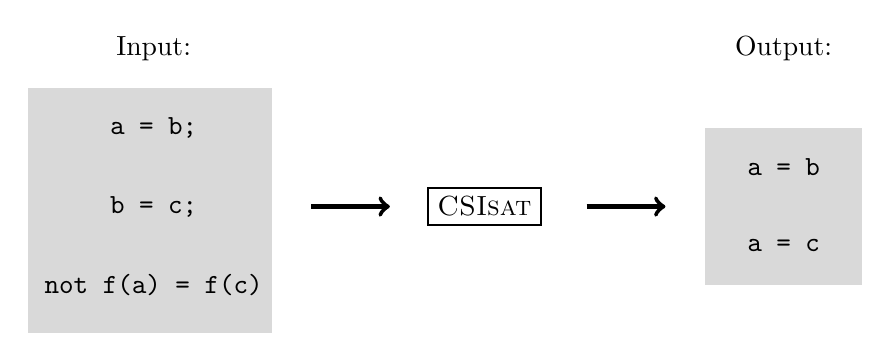
\begin{tikzpicture}[auto, node distance=3cm, semithick]
  \fill[black!15!white] (-1.6,-0.6) rectangle (1.5,2.5);
  \node [draw=none] (in) at (0,3) {Input:};
  \node [draw=none] (x1) at (0,2) {{\tt a = b;}};
  \node [draw=none] (x2) at (0,1) {{\tt b = c;}};
  \node [draw=none] (x3) at (0,0) {{\tt not f(a) = f(c)}};

  \visible<2->{
    \draw [->, ultra thick] (2,1) to (3,1);
    \node [thick,draw] (cs) at (4.2,1) {\csisat{}};
  }
  
  \visible<3->{
    \draw [->, ultra thick] (5.5,1) to (6.5,1);
    \fill[black!15!white] (7,0) rectangle (9,2);
    \node [draw=none] (out) at (8,3) {Output:};
    \node [draw=none] (i1) at (8,1.5) {{\tt a = b}};
    \node [draw=none] (i2) at (8,0.5) {{\tt a = c}};
  }

  \end{tikzpicture}
  \end{figure}
\end{frame}

\section{How \csisat{} works ?}
%\begin{frame}
%  \frametitle{General}
%  \csisat{} combines several known algorithms and provides them as open-source software.
%  \vspace{5pt}
%
%  \begin{tabular}{lcl}
%    Interpolation for EUF & $\rightarrow$ & McMillan 05\\
%    Interpolation for LA & $\rightarrow$ & Rybalchenko et al. 07\\
%    Interpolation using Nelson-Oppen & $\rightarrow$ &   Yorsh et al. 05\\
%     & + & Rybalchenko et al. 07\\
%    Interpolation with a resolution proof & $\rightarrow$  & Yorsh et al. 05
%  \end{tabular}
%
%\end{frame}

\begin{frame}
  \frametitle{Architecture}
  \begin{enumerate}
    \item Generating a resolution proof of unsatisfiability.
    \item<3-> Constructing the interpolant.
  \end{enumerate}

  \begin{figure}
  \centering
  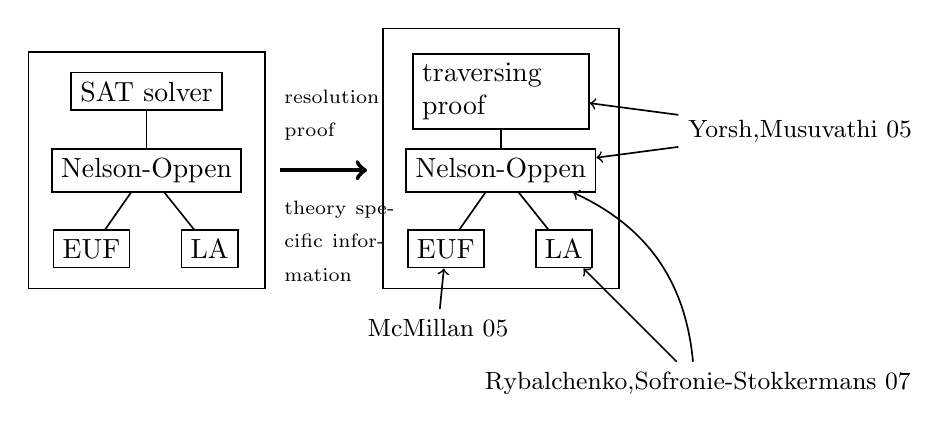
\begin{tikzpicture}[auto, node distance=3cm, semithick]

  \draw (-0.5,-0.5) rectangle (2.5,2.5);
  \node [draw] (sat) at (1,2) {SAT solver};
  \node [draw] (no) at (1,1) {Nelson-Oppen};
  \node [draw] (la) at (1.8,0) {LA};
  \node [draw] (euf) at (0.3,0) {EUF};
  \path (sat) edge (no);
  \path (no) edge (la);
  \path (no) edge (euf);

  \visible<2->{
    \draw [->, ultra thick] (2.7,1) to (3.8,1);
  }
  \visible<2>{
    \node [text width=15mm] (rp) at (3.5,1.7) {\scriptsize resolution proof};
    \node [text width=15mm] (uc) at (3.5,0.1) {\scriptsize theory specific information};
  }
  
  \visible<3->{
    \draw (4,-0.5) rectangle (7,2.8);
    \node [draw,text width=2cm] (trav) at (5.5,2) {traversing proof};
    \node [draw] (no2) at (5.5,1) {Nelson-Oppen};
    \node [draw] (la2) at (6.3,0) {LA};
    \node [draw] (euf2) at (4.8,0) {EUF};
    \path (trav) edge (no2);
    \path (no2) edge (la2);
    \path (no2) edge (euf2);
  }

  \visible<4->{
    \node (yorsh) at (9.3,1.5) {{\small Yorsh,Musuvathi 05}};
    \draw [->] (yorsh) edge  (trav);
  }

  \visible<5->{
    \node (rybal) at (8,-1.7) {{\small Rybalchenko,Sofronie-Stokkermans 07}};
    \draw [->] (yorsh) edge  (no2);
    \draw [->] (rybal) edge [bend right] (no2);
  }
  
  \visible<6->{
    \node (mcmill) at (4.7,-1) {{\small McMillan 05}};
    \draw [->] (mcmill) edge (euf2);
  }
  
  \visible<7->{
    \draw [->] (rybal) edge  (la2);
  }

  \end{tikzpicture}
  \end{figure}
\end{frame}

\section*{Conclusion}
\begin{frame}
  \frametitle{Performance}
  
\begin{figure}
{\footnotesize
\centering
\begin{tabular}{|l|rrrr|}
  \hline
  Program ~~~~~~~ &   \#queries  & ~ \foci{} & ~ \clpprover{}  & \textbf{~\csisat{}}     \\
  \hline
  \hline
  \blast{}\footnote{\url{http://mtc.epfl.ch/blast/}} & & & & \\
  floppy              &   235        & 1.17\,s    &  1.55\,s         & \textbf{0.55\,s}        \\
  cdaudio             &   130        & 0.60\,s    &  0.70\,s         & \textbf{0.26\,s}         \\
  ssh                 &  6881        & 29\,s      & ---              & \textbf{17\,s}         \\
  \hline
  \armc{}\footnote{\url{http://www.mpi-sws.mpg.de/~rybal/armc/}} & & & & \\
  magill      &  9860        & ---        & 30\,s            & \textbf{21\,s}         \\
  \hline
\end{tabular}
}
\end{figure}

\vspace{1cm}
{\footnotesize
Related work: the new version of \mathsat{} [CAV 08] can generate interpolants.
}

\end{frame}

\begin{frame}
  \frametitle{Try it out! }
  \csisat{} is freely available online:
  \begin{itemize}
    \item Project web page:\\ 
          \url{http://www.cs.sfu.ca/~dbeyer/CSIsat}
    \item Sources and bug reports:\\ 
          \url{http://csisat.googlecode.com}
    \item Feedback very welcome!
    \item[]
    \item Questions?
  \end{itemize}
\end{frame}
%-------------------------------------------------------------------------
%\bibliography{../../bib/sw,../../bib/tah}
%\input{main.bbl}

\end{document}


\end{document}


\end{document}


\end{document}
